\section{Analisi dei requisiti}
L'obiettivo da raggiungere era quello di realizzare un tool che, attraverso una UI semplice e gradevole, ci permettesse di interrogare la blockchain in base a parametri, valori e regole arbitrarie.

\section{Scelte fatte}

Il primo strumento scelto è stato il framework di sviluppo: Angular;
la scelta è stata semplice in quanto è uno dei migliori strumenti sul mercato, ha una grande community, è ben documentato è semplice da usare e permette di tenere il codice pulito e ben strutturato.

\vspace{0.5cm}

Successivamente abbiamo scelto web3.js come "accesso" alla blockchain;
avevamo diverse alternative come effettuare le chiamate RPC esposte dal nodo Ethereum a mano ma questa opzione ci sembrava particolarmente costosa per i tempi di sviluppo,
oppure avremmo potuto leggere i dati direttamente dal database locale del nodo ma in questo caso lo sviluppo sarebbe stato complesso, lungo e soprattutto avremmo ottenuto una soluzione estremamente "verticale" e non modulare.
Un'altra opzione era quella di appoggiarci a servizi terzi come ad esempio Etherscan che espone alcune api per leggere dati dalla blockchain:
pur garantendoci il vantaggio di non doverci occupare della gestione del nodo locale ci sembrava comunque una solzione non modulare ed inoltre queste api, essendo gratuite, sono filtrate e ci sono dei limiti di traffico da rispettare.
Web3.js ci garantisce modularità, è molto semplice da usare e completamente compatibile con Angular.

\vspace{0.5cm}

L'ultimo strumento scelto è stato Parity che è uno dei numerosi client di Ethereum. \'E stato scelto perchè uno dei più famosi ed usati.

\section{Descrizione progetto}
Il primo passo dello sviluppo è stata la modellazione delle entità principali del dominio: account, blocchi e transizioni.
\begin{lstlisting}
export interface Transaction {
  hash: string;
  nonce: number;
  blockHash: string;
  blockNumber: number;
  transactionIndex: number;
  from: string;
  to: string;
  value: BigNumber;
  gas: number;
  gasPrice: BigNumber;
  input: string;
}
\end{lstlisting}
Nel listato precedente possiamo vedere la modellazione delle transizioni.
Alcune proprietà sono di tipo BigNumber: questo tipo è definito dall'omonima libreria javascript ed è usata quando è necessario lavorare con numeri a precisione arbitraria.

Dopo aver modellato l'ambiente sono stati implementati i servizi, ovvero quei componenti software che si occupano di implementare la logica di business.
Ogni servizio implementa un'interfaccia per rendere il codice modulare e più facilmente usabile con la dependency injection.
In questo caso sono stati implementati:
\begin{itemize}
    \item {\bfseries Localdataprovider}: il suo compito è quello di recuperare i dati dalla blockchain e fornirli, attraverso un observable, ad altri componenti software.
    Ecco i metodi più interessanti.

    \begin{lstlisting}
      getBlocks(start: number, end: number): Observable<Block> {
        return new Observable((observer) => {
          for (let i = start; i < end; i ++) {
            setTimeout((() => {
              const block = this.web3.eth.getBlock(i) as Block;
              block.difficulty = block.difficulty.dividedBy(new BigNumber('1000000000000000000'));
              block.totalDifficulty = block.totalDifficulty.dividedBy(new BigNumber('1000000000000000000'));
              observer.next(block);
              if (i + 1 === end) {
                observer.complete();
              }
            }), this.delayInms);
          }
        });
      }

      getTransactions(start: number, end: number): Observable<Transaction> {
        return new Observable((observer) => {
          for (let j = start; j < end; j ++) {
            const block = this.web3.eth.getBlock(j) as Block;
            if (!block) {
              continue;
            }

            for (let i = 0; i < block.transactions.length; i ++) {
              setTimeout((() => {
                const hash = block.transactions[i];
                const item = this.web3.eth.getTransaction(hash) as Transaction;
                item.value = item.value.dividedBy(new BigNumber('1000000000000000000'));
                observer.next(item);

                if (j + 1 === end && i + 1 === block.transactions.length) {
                  observer.complete();
                }
              }), this.delayInms);
            }
          }
        });
      }
    \end{lstlisting}
    In questo servizio viene usato web3.js mentre il resto dell'applicazione praticamente non ha idea di come i dati vengono recuperati.
    Possiamo notare anche una particolarità di web3.js: i valori di tipo BigNumber restituiti sono misurati in 'wei' e non in ETH, per questo viene effettuata la conversione dividendo per 1000000000000000000.
    Inoltre è possibile vedere che viene ritornato un observable e i dati vengono serviti in modo asincrono all'observer man mano che vengono recuperati.

    \item {\bfseries Dataprojector}:
    Questo servizio invece si occupa di effettuare la 'proiezione', usando l'accezione tipica del mondo dei database, dei dati.
    Sostanzialente dato un oggetto e una lista di proprietà ritorna i valori di quelle proprietà dell'oggetto.
    Ecco il metodo più interessante di questo componente:
    \begin{lstlisting}
        getValues(source: any, properties: string[]): any[] {
            if (!source || !properties) {
              return [];
            }

            const values: any[] = [];
            properties.forEach(prop => {
                values.push(source[prop as string]);
            });
            return values;
        }
    \end{lstlisting}

    \item {\bfseries Dataselector}:
    Anche in questo caso il nome è preso in prestito dal mondo SQL dato che questa classe si occupa di effettuare la selezione dei dati;
    quindi si occupa di verificare se un determinato oggetto rispetta delle regole.
    Le regole in questione sono state formalizzate sotto forma di 'Constraint' in questo modo:

    \begin{lstlisting}
        export class Constraint {
            property: string;
            operator: string;
            value: any;
            logicalOperator?: LogicalOperator = null;
        }
    \end{lstlisting}

    Questo invece è il metodo che ricevuta una lista di oggetti ed una lista di regole, filtra solo gli oggetti che seguono le regole specificate.
    \begin{lstlisting}
        filter(source: any[], constraints: Constraint[]): any {
            if (!source || source.length <= 0) {
                return [];
            }

            if (!constraints || constraints.length <= 0) {
                return source;
            }

            const result = [];
            for (let i = 0; i < source.length; i++) {
                const item = source[i];
                if (this.respectsAllConstraints(item, constraints)) {
                    result.push(item);
                }
            }

            return result;
        }
    \end{lstlisting}

    \item {\bfseries Camquerist}:
    L'ultimo servizio implementato è stato il servizion che si occupa di gestire e coordinare tutti quelli che abbiamo visto in precedenza.
    Praticamente recupera i dati dal data provider, li filtra con il data selector e li proietta affidandosi al data projector.
    La sua utilità è quella di fornire un unico punto di accesso per far partire la query nascondendo il coordinamento dei diversi servizi alle classi che lo utilizzano.

\end{itemize}

Per quanto riguarda la UI abbiamo usato i componenti di Angular/Material.
Di seguito la schermata principale del nostro strumento in cui possiamo vedere diversi componenti tipici del Material design:
si possono vedere la toolbar blu in alto, il burger-menu le cardview che contengono le diverse sezioni delle query ed infine il floating button per lanciare l'esecuzione dell'interrogazione.

\begin{center}
    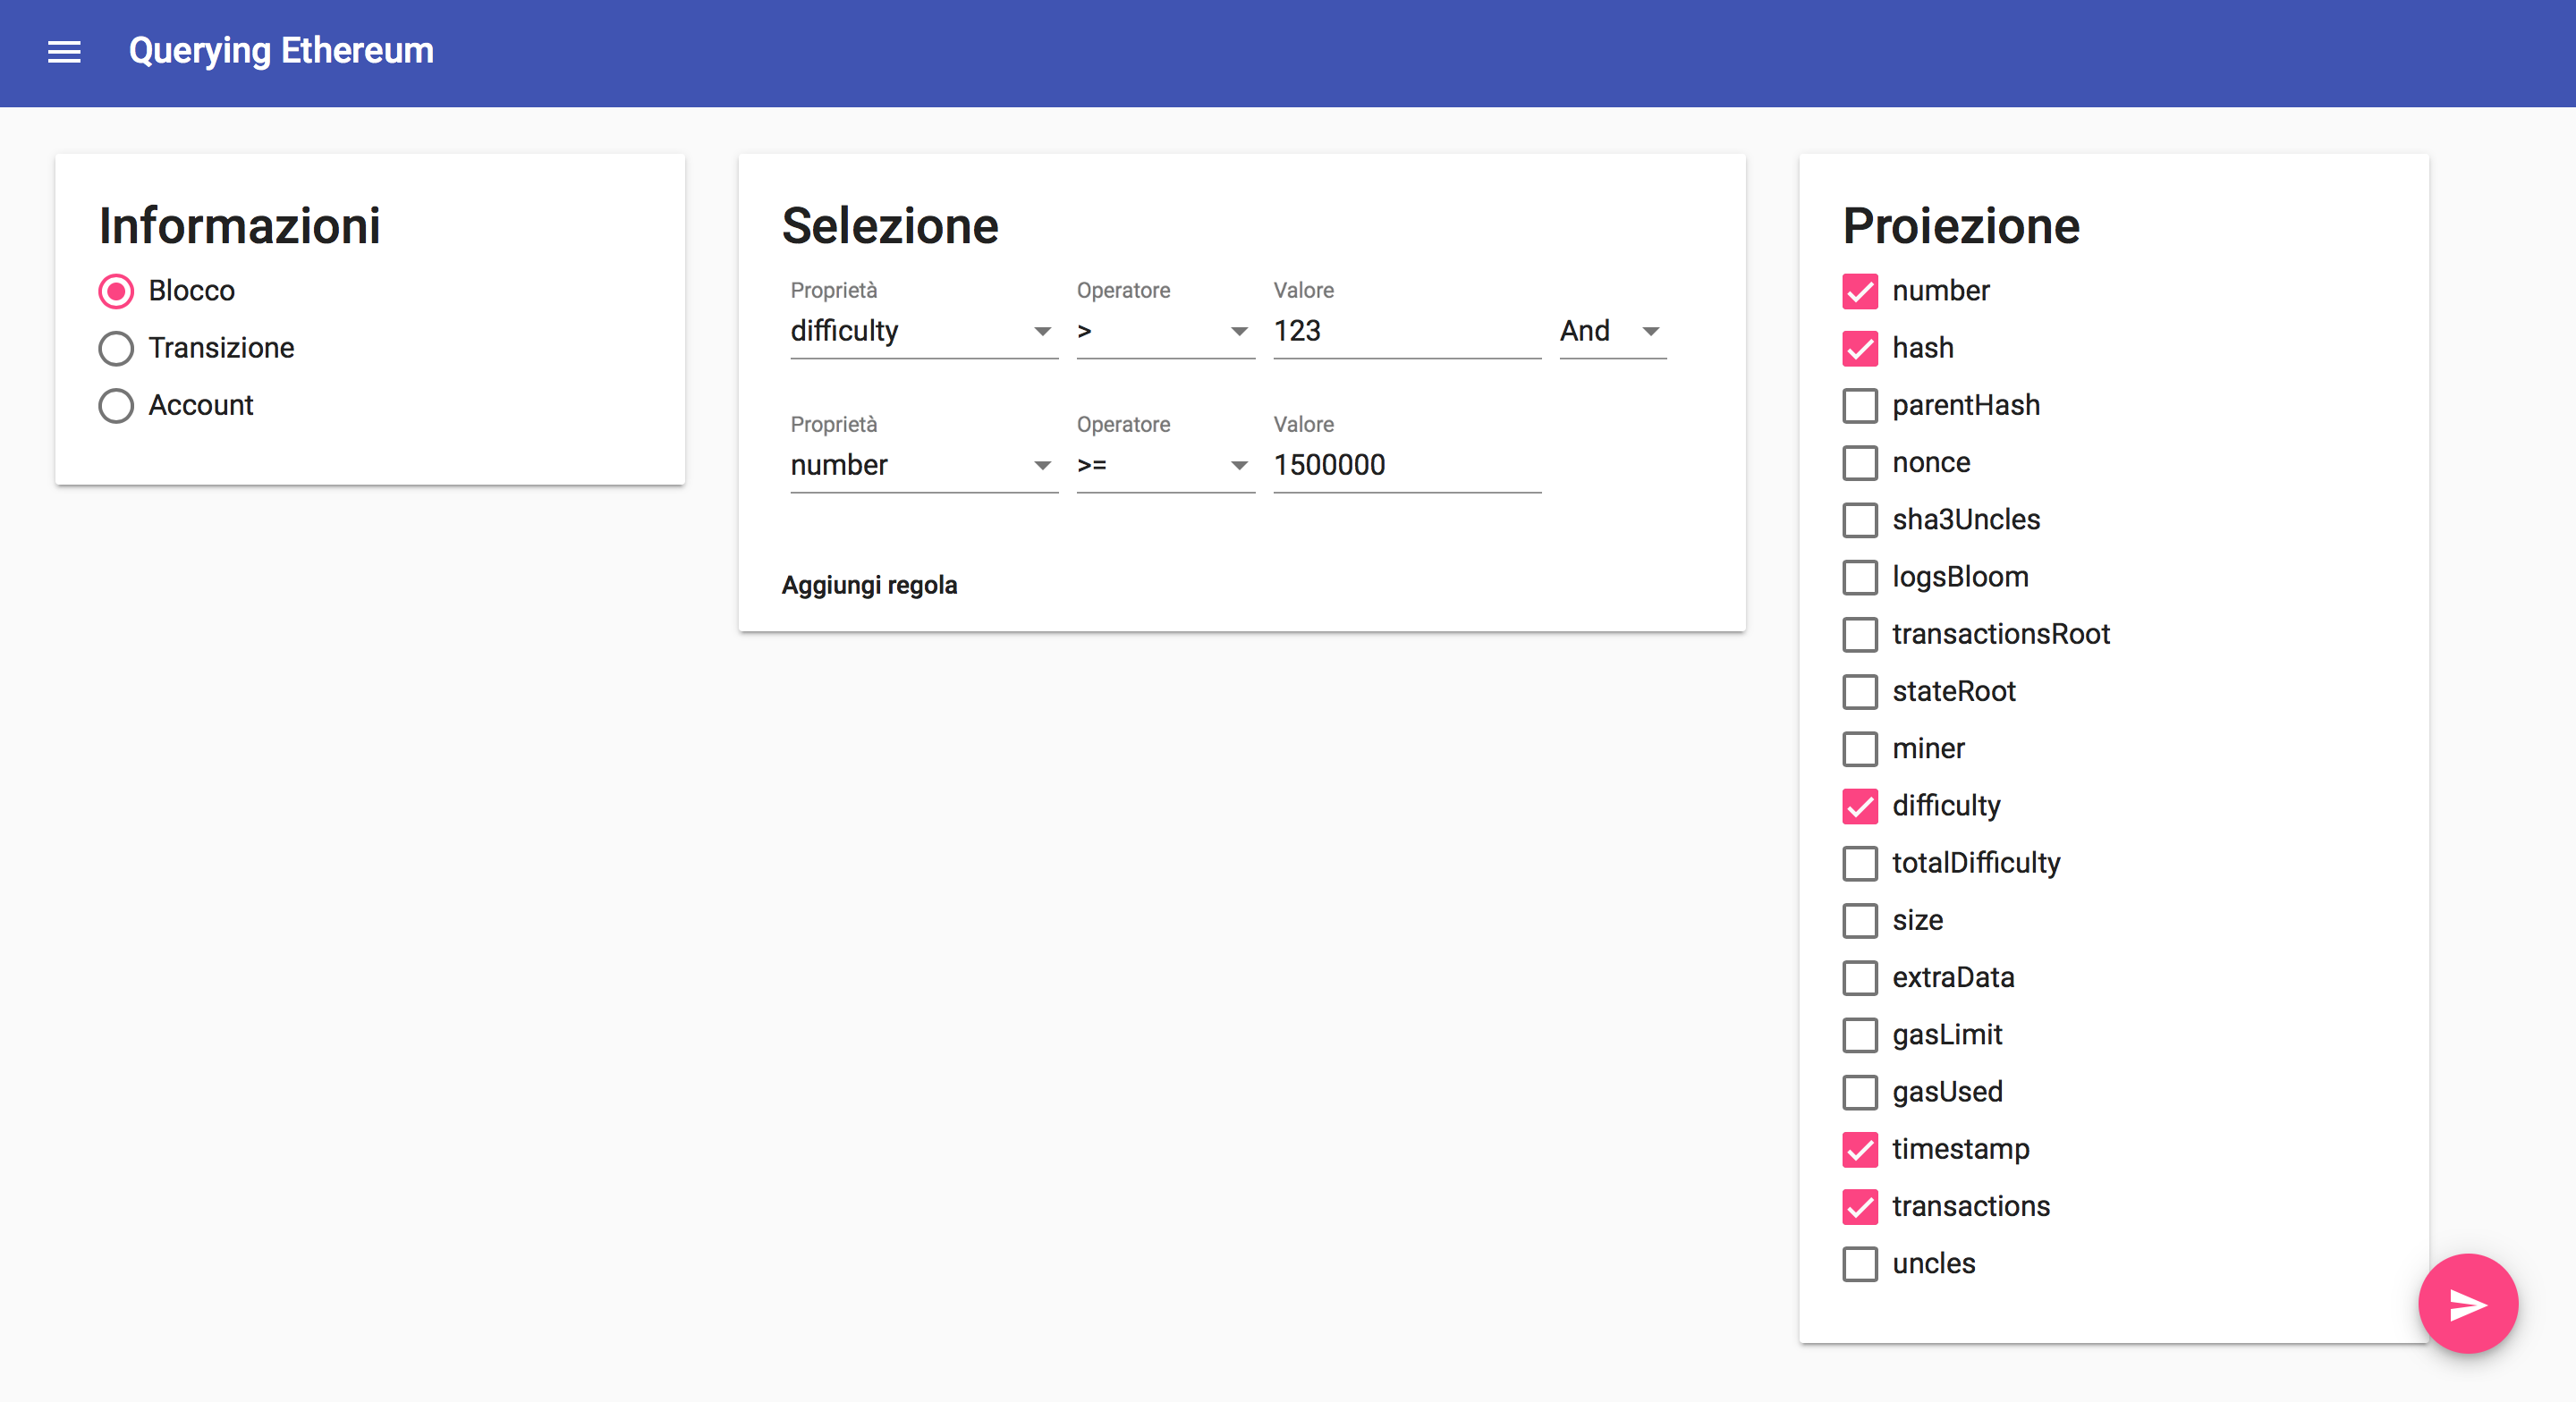
\includegraphics[scale=0.3]{screen.png}
\end{center}

\section{Problemi incontrati}
Dopo lo studio iniziale ed una prima implementazione grossolana del progetto abbiamo riscontrato un problema che avevamo trascurato:
effettuare query all'intera blockchain è un'operazione molto costosa dal punto di vista computazionale e di conseguenza lenta (potenzialmente anche diversi giorni).

Indagando abbiamo stimato che usando web3.js ogni chiamata alla libreria impiega mediamente 100 ms:
prendendo il valore da solo è un tempo più che accettabile il problema nasce dal fatto che web3.js mappando le chiamate RPC esposte dai nodi Ethereum
fornisce delle api estremamente granulari e specifiche che non permettono alcuna aggregazione di dati.
Questo significa che è necessario effettuare un gran numero di chiamate per poter ottenere dati aggregati:
per dare un'idea della cardinalità delle chiamate necessarie basti pensare che per ottenere le transizioni di 50 blocchi sono necessarie (mediamente) diverse migliaia di chiamate (si può immaginare per 10000 o più blocchi).

Ovviamente questo non è un problema evitabile essendo una conseguenza della natura stessa della Blockchain ma abbiamo trovato una soluzione che ci permette di mitigare il probelma rendendo usabile lo strumento anche con tempi lunghi.

\vspace{0.5cm}

Ci siamo imbattuti poi in un nuovo problema. Andando a fare così tante operazioni al secondo la CPU della macchina che eseguiva l'applicazione raggiungeva presto il 100\% di utilizzo.
Questo oltre a rallentare il sistema operativo, surriscaldare la macchina fisica portava anche la nostra applicazione a freezarsi, ovvero a non rispondere più all'interazione con l'utente.

\section{Soluzioni adottate}

Per risolvere il problema della durata della query abbiamo valutato di tornare indietro sulla scelta di web3.js.
Abbiamo rivalutato di nuovo le varie possibilità ancora una volta ma la scelta è restata la medesima in quanto ognuna delle altre possibilità aveva delle controindicazioni.
L'unica soluzione percorribile sarebbe stata quella di creare un servizio per l'indicizzazione della Blockchain:
avrebbe di sicuro migliorato di gran lunga le performance ma oltre ad essere un progetto piuttosto complesso (gestione degli errori, continua sincronizzazione con la blockchain, sincronizzazzione incrementale ...)
significava realizzare una seconda applicazione il cui 'compito' esulava dagli obbiettivi del Project (non ci interessa indicizzare la Blockchain!).

La soluzione adottata invece è stata di natura puramente tecnica:
accettando il fatto che query su tanti blocchi sono lente possiamo però comunque rendere lo strumento usabile mostrando all'utente i risultati parziali della query e dandogli feedback sul fatto che la query è ancora in esecuzione.
L'utente sa che la query è in esecuzione attraverso un indicatore di lavoro e ma man mano che vengono trovati record che rispettano la query vengono mostrati all'utente.
Questo migliora notevolmente l'esperienza e di conseguenza l'usabilità.
Praticamente l'esecuzione della query ora è uno streaming di dati sotto forma di pipe.
Dal punto di vista tecnico questa modifica è stata possibile grazie all'uso degli Observable e della libreria Rxjs.

\vspace{0.5cm}

Il secondo problema invece è stato risolto utilizzando la funzione Javascript 'setTimeout'.
Sostanzialmente invece che eseguire subito la chiamata a web3.js in modo sincrono la facciamo in un secondo momento dando modo alla CPU di fermarsi o dedicarsi ad altri processi.
